\chapter{LinkedPipes Applications}
\label{chap:num_1}

In this chapter, the main functional requirements of LinkedPipes Applications are briefly described. This provides a better understanding about the platform and consequently serves as an introduction to defining the functional requirements of the \lpa{}.

%  TODO : describe components of the architecture

As mentioned in previous chapters, the overall goal on LinkedPipes Applications is to create a web-based tool that would allow generation of interactive visualizations by some domain expert, that can then be embedded in an online article or on another web page or perhaps simply accessed as a standalone page.

The following section uses the various acronyms and terms specific to Semantic Web: 

\begin{itemize}
    \item \gls{IRI} -- IRIs are a superset of Uniform Resource Identifiers (URI) which allow for the inclusion of Unicode characters such as Chinese or Cyrillic symbols in the identifier string. IRIs are extensively used as entity identifiers in Linked data.
    \item SPARQL endpoint is an interface through which a user can query and inspect data stored in a particular RDF data storage.
    \item Dataset is a collection of data available for access or download from a single data store such as a catalog or a SPARQL endpoint.
    \item TTL -- short for Terse RDF Triple Language, one of the RDF serialization formats.
\end{itemize}

\section{Components overview}

At the lower level, the \lpa{} is a bundle of various complex services and database solutions communicating between each other in docker environment. 

\begin{figure}[h]
    \centering
    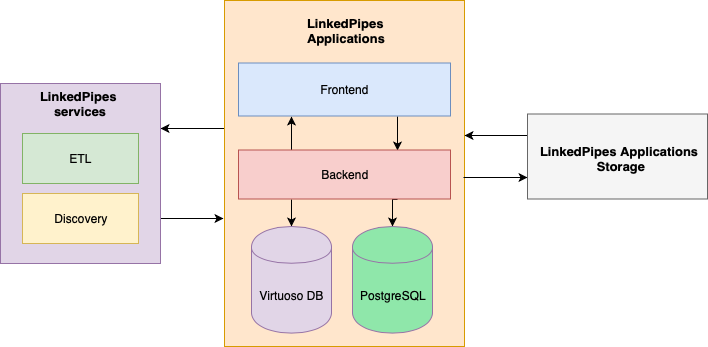
\includegraphics[width=14cm]{lpa_highlevel_architecture.png}
    \caption{High-level overview of LinkedPipes Applications Platform}
    \label{fig:lpa-high-level-arch}
\end{figure}

Generally, we can categorize it into three main parts: 

\begin{itemize}
    \item \textbf{\lpa{}} - the main platform from LinkedPipes bundle, and the main stakeholder for \lpas{} project. Combines multiple database solutions for LinkedData, conventional SQL for storing user related records and implementation of a backend and frontend for creating applications.
    \item \textbf{LinkedPipes Services} - a set of external services provided from LinkedPipes bundle that \lpa{} heavily utilizes. Provides a toolset for identifying how linked data can be discovered, extracted, transformed and loaded into an RDF file for further processing.
    \item \textbf{\lpas{}} - the main goal of the following thesis and a functional storage solution for \lpa{} platform. Contains a set of API controllers and managers that allow users of \lpa{} to store and share their applications in a secure and decentralized way. Consecutive chapters will provide a detailed overview of an architecture and implementational details.
\end{itemize}

\subsection{\lpa{}}

\subsubsection{Frontend}

\subsubsection{Backend}

\subsubsection{Virtuoso DB}

\subsubsection{PostgreSQL} 

\subsection{LinkedPipes Services} 

\subsubsection{Discovery} 

\subsubsection{ETL} 

\subsection{\lpas{}}

\section{Functional requirements}

The following sections describes the main functional requirements defined for the \lpa{}. 

\subsection{User authentication}

The user of the platform should be able to register an account in the application, log in and log out. Moreover, once logged in, the platform should be provide functionality to create, configure and publish applications visualizing LinkedData. However, to view an application, it is not necessary to be logged in or even registered.

\subsection{Create Application}

The Create Application functionality could be described as a core feature of the LinkedPipes Application.

The platform needs to provide the a tooling to specify the data sources to be utilized so that an instance of an interactive application would be created based on provided data sources. In addition to that, there needs to be four ways to provide the data source:

\begin{itemize}
\item Provide a set of dataset \acrshort{IRI}s which the tool will de-reference to get the dataset.
\item Specify a \acrshort{SPARQL} endpoint from which data will be queried and extracted.
\item Upload a file in \acrshort{TTL} format, containing data source specifications.
\item Use some sample dataset provided by the tool
\end{itemize}

\subsection{Configure Application}

After the creation of the application, platform also need to provide functionality to configure previously created applications. Each application, depending on the visualization, will have particular settings that can be set. Furthermore, users must be able to control, with the use of filters, which data is to be used and displayed. The available filters should be automatically derived based on the properties and semantics of the data. 

The set of configure operations for filters can be described as follows:

\begin{itemize}
\item Removing whole data filters to ignore the values of specific data properties.
\item Removing selected values of some filters.
\item Setting fixed values for some filters.
\item Set/change a name for the application.
\end{itemize}

\subsection{Publish Application}

Another important requirement is an ability to publish the application and make it publically available for sharing the visualization to anyone via the permanent link. Furthermore, when a third party accesses this \textit{permalink}, the browser should open the LinkedPipes Applications website with the respective application opened, as configured by the publisher.

Besides, when publishing an application I want the tool to offer the possibility to choose one of the below two settings:

\begin{itemize}
\item Use and display cached data, making the published application a fixed view.
\item Regularly refresh the data from the previously chosen data sources of the interactive application.
\end{itemize}

The tool will also need to provide the ability to embed the published view into a data journalist's web page, for example, using an iFrame.

\subsection{Store Application}

Since published applications require to be publically accessible to anyone, the platform needs to have a functionality to persist the configurations of the applications in a secure way. Moreover, the configurations for most of the published applications are represented as LinkedData, therefore the persistent storage tooling needs to be optimized for files in RDF format. 
User needs to be able to browse the stored and published applications and optionally allow other people to collaborate or edit a specific shared application. 

% A detailed overview of the solution as well as the overview of current alternatives to \solid is provided in the consecutive chapters of this thesis. 